%!TEX root = ../thesis.tex
%*******************************************************************************
%****************************** Third Chapter **********************************
%*******************************************************************************
\chapter{Developing an integrated reference for automatic cell type annotation} \label{chap:CT_method}

% **************************** Define Graphics Path **************************
\ifpdf
    \graphicspath{{Chapter3/Figs/Raster/}{Chapter3/Figs/PDF/}{Chapter3/Figs/}}
\else
    \graphicspath{{Chapter3/Figs/Vector/}{Chapter3/Figs/}}
\fi
The widespread adoption of single-cell sequencing technologies has revolutionised the molecular profiling of cells. The use of these methods allows us to understand the building blocks of tissues at an unprecedented resolution. As further human tissues are examined, a catalog of cell types and their gene expression profile can be compiled from published data. Such compilation, covering a broad variety of organs and obtained using different methodologies, can provide a reference to which newly collected data can be compared for immediate annotation, while in parallel revealing the underlying relationships between cell populations across the organism.

This chapter outlines the development of \textit{CellTypist} - an integrative reference of cell types based on single-cell transcriptomic data. The \textit{CellTypist} pipeline relies on predictive models to integrate data from different sources, and allows for automatic and unbiased annotation of scRNA-seq datasets. Additionally, integration of data from numerous sources can inform on cell type similarity, and thus serve as a framework for an expression-based cell type ontology.

This project was initially conceived together with Valentine Svensson while he was part of the Teichmann group. The pipeline here outlined serves as the basis for the analyses performed in Chapter~\ref{chap:CT_bio}.


\section{Introduction}
\label{section3.1}
% cataloguing all cell types
The aim of classifying and characterising all different types of cells that compose the various anatomical regions has been present ever since it was first postulated that all living organisms are composed of cells~\citep{schwann_microscopical_1847}. For the greater part of the history of cell biology, cells have been characterised and identified based on their physical appearance~\citep{mazzarello_unifying_1999}. The development of immunohistochemistry~\citep{coons_immunological_1941}, and later its combination with the large throughput provided by flow cytometry and FACS~\citep{hulett_cell_1969,bonner_fluorescence_1972}, started the current trend of molecular definition of cell types. More recently, developments in single-cell sequencing have enabled unbiased and high-throughput assessment of cell types through transcriptomic profiling~\citep{svensson_exponential_2018}. A few individual works have aimed at profiling cell types across most tissues of an organism~\citep{fincher_cell_2018,plass_cell_2018,han_mapping_2018,noauthor_single-cell_2018}. Other more complex and detailed cellular census have been done for individual tissues, and large consortia have been established to aggregate some of these datasets and establish guidelines and collaborations to identify all cell types across an organism~\citep{regev_human_2017}.

% integration methods, classification methods, comparison
Individually, studies using scRNA-seq have provided crucial insights into cell biology. Nonetheless, the data generated can often be reused for new purposes, either on its own to extract new conclusions, or through combination or comparison with novel data. To combine scRNA-seq datasets, batch correction and batch alignment methods seek to either correct gene expression values accounting for technical metadata~\citep{ritchie_limma_2015,johnson_adjusting_2007,buettner_f-sclvm:_2017,haghverdi_batch_2018,buttner_test_2019}, or place cells from different batches, technologies and datasets in a common manifold, allowing joint clustering and pseudotime analysis~\citep{butler_integrating_2018,polanski_bbknn:_2019,hie_efficient_2019,korsunsky_fast_2018,stuart_comprehensive_2019}. Conversely, comparison between scRNA-seq datasets aims to impart the knowledge gained from one dataset into another, usually through classification models. Various methods have been developed to compare cell types (and indeed other labels) across datasets (reviewed in Chapter~\ref{section1.3}, Table~\ref{table:tab_1_2}). Nonetheless, while these tools are highly effective at annotating new data using specific datasets, their scope will be limited to the dataset chosen as a reference.

% short description of the chapter
%% mention nomenclature: cell types - prior annotation; clusters - any derived, not named labelling. CellTypist, by default, uses CLUSTERS
To address the need for a reference that can allow fast and automatic annotation across tissues, we have developed \textit{CellTypist}, a pipeline for integration and classification based on logistic regression classifiers. Providing this pipeline with a broad collection of datasets creates an unbiased cell identity reference to be used in novel datasets. While previous work has been developed for well annotated mouse data  using a neural network-based classifier~\citep{alavi_web_2018}, \textit{CellTypist} can leverage data with different levels of annotation, focusing on providing broad identifiers for cells based on a reference from pooled data.

\begin{figure}[ht!]
    \centering    
    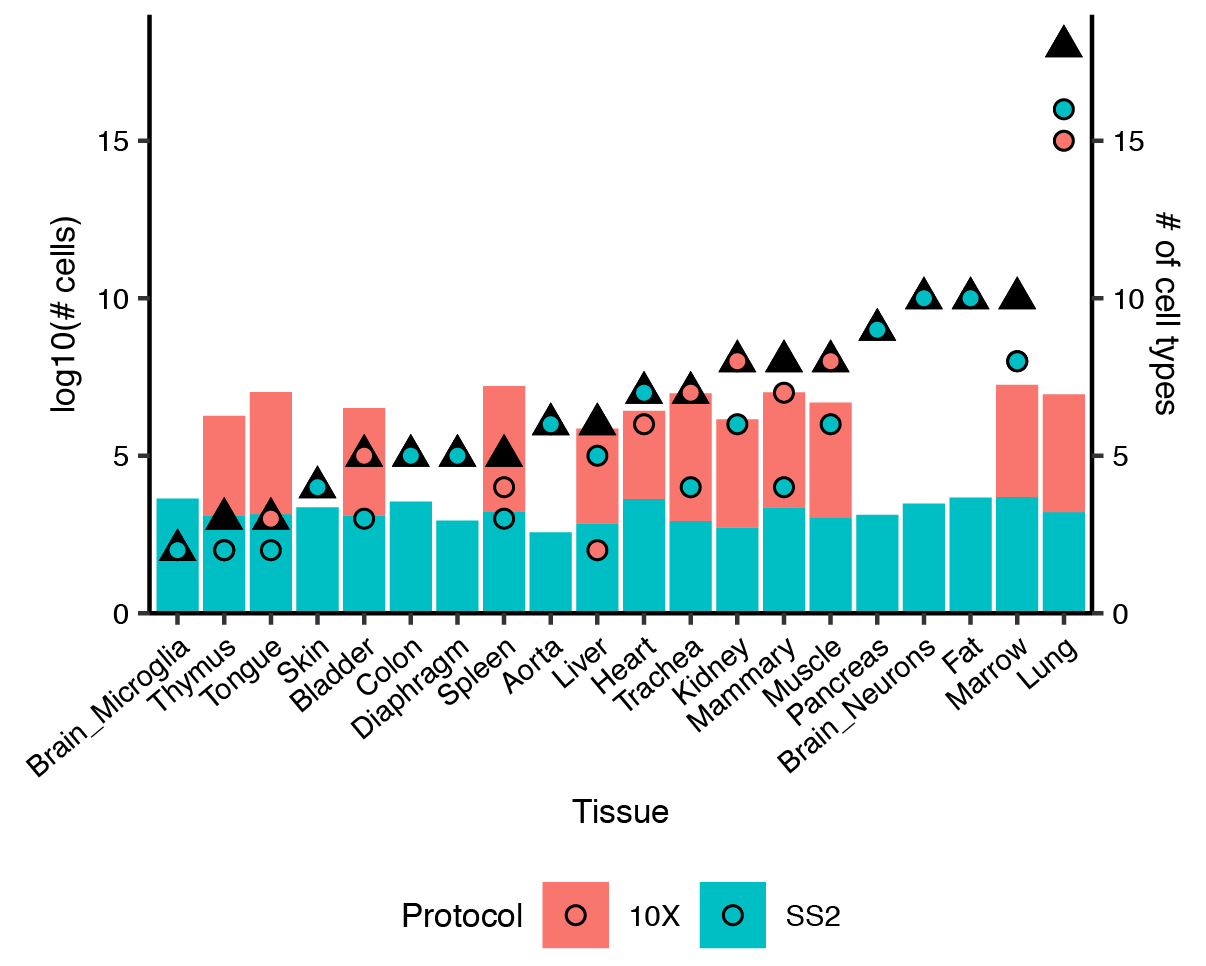
\includegraphics[width=1.0\textwidth]{Chapter3/Figs/countsCTCells_TabulaMuris.png} % change word in curlies to change figure
    \caption[Cell numbers in the \textit{Tabula Muris} dataset]{\textbf{Cell numbers in the \textit{Tabula Muris} dataset} \newline Bars show number of cells (left y axis) collected from different tissues (x axis), split by scRNA-seq protocol (colour). Points show the number of cell types (right y axis) identified by protocol (coloured circles) or their union (triangle). 10X - Chromium (10X Genomics) protocol; SS2 - Smart-seq2 protocol.}
    \label{fig:chap3_tmcounts}
\end{figure}

This chapter discusses the organisation of the \textit{CellTypist} pipeline, and explores its strengths and caveats. Evaluation of the pipeline will be performed on the \textit{Tabula Muris} data~\citep{noauthor_single-cell_2018}, summarised in Figure~\ref{fig:chap3_tmcounts}. Despite coming from a sole publication, this dataset has the advantage that it was generated in highly controlled conditions, spans 20 tissues, and includes a detailed and robust cell type annotation to which the clusters that result from integration using \textit{CellTypist} can be compared. The next Chapter will further explore the biological insights extracted from a collection of published human data from various sources, and how it can be used to interpret new data.


\nomenclature[z-SS2]{SS2}{Smart-seq2}

\section{Methodology and Results}
\label{section3.2}
\subsection{per-tissue clustering and cell type comparison}
\label{section3.2.1}
Reference data processing with \textit{CellTypist} follows three major steps. First, the data collected follows a procedure for uniform per-tissue processing (Figure~\ref{fig:chap3_pertiss}A). Next, the clusters determined in each tissue are matched across the whole dataset (Figure~\ref{fig:chap3_combcl}A). Lastly, the combined clusters are used as labels to train a logistic regression classifier using the complete data collection (Figure~\ref{fig:chap3_model}A).

Most studies using scRNA-seq profile cellular heterogeneity in a given biological sample, which often results in reporting the cell types or cell states present. While this is clearly displayed in the figures from these studies, this information in not always supplied in a machine-readable format, associated with either the raw sequencing reads or the quantified gene expression. Furthermore, most annotations do not follow a uniform, controlled vocabulary~\citep{bard_ontology_2005}, and is often done at varying resolutions depending on the focus of the study or the breadth of the dataset.

\textit{CellTypist} starts by splitting the collected data by tissues, grouping together data from different studies that profile the same body part, even if using distinct scRNA-seq protocols (Figure~\ref{fig:chap3_pertiss}A). At this stage, data from each tissue is processed following a uniform workflow using scanpy~\citep{wolf_scanpy:_2018}. Gene expression counts are normalised by their total counts and log transformed, and different datasets are batch aligned using BBKNN~\citep{polanski_bbknn:_2019} - in \textit{Tabula Muris}, different protocols are treated as independent data. Lastly, clustering at varying resolutions using the Leiden algorithm~\citep{traag_louvain_2019} is performed. This processing is executed to ensure that all tissues are similarly treated, regardless of the level of annotation, and to allow unannotated data to be included and bolster \textit{CellTypist}'s training data.

\begin{figure}[pht!]
    \centering    
    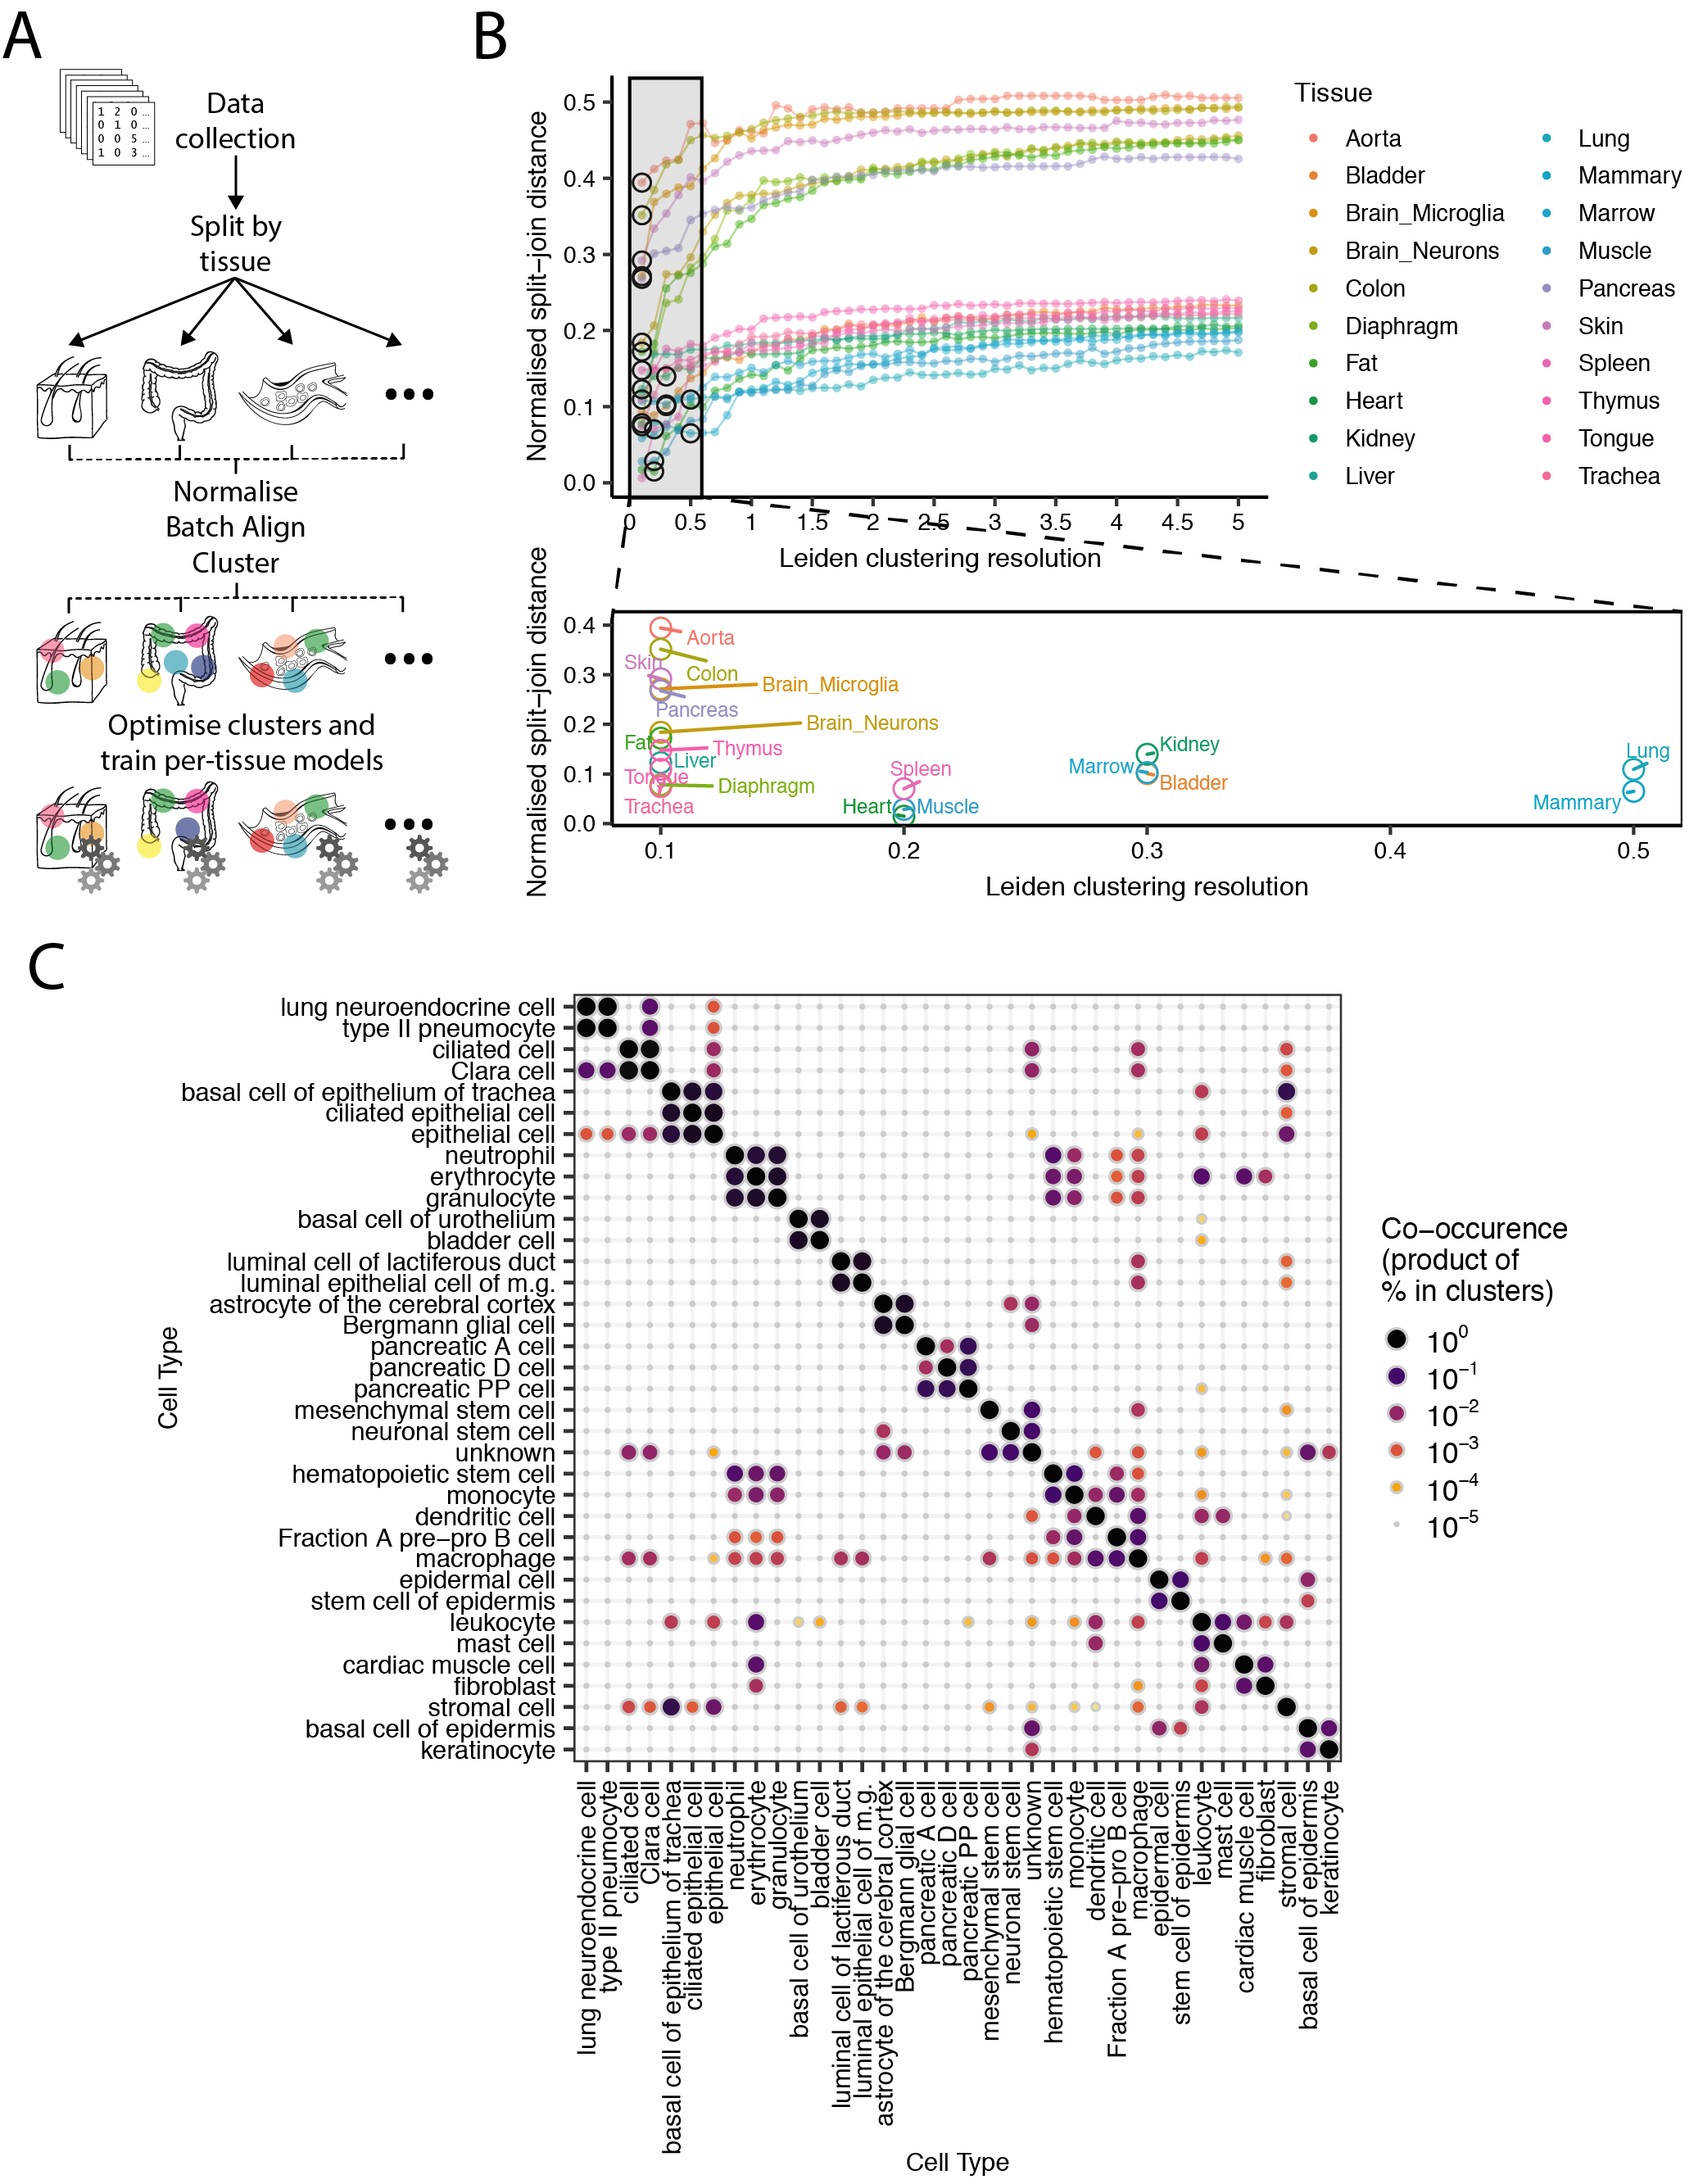
\includegraphics[width=1.0\textwidth]{Chapter3/Figs/chap3_TMperTissue.png} % change word in curlies to change figure
    \caption[Data reprocessing per-tissue]{\textbf{Data reprocessing per-tissue}\newline\textbf{(A)} Pipeline for initial data processing. Data collected is split into tissue, followed by integration of different datasets (in \textit{Tabula Muris}, different protocols), and clustered to optimally match existing cell type annotations. (Continued on the following page.)}
    \label{fig:chap3_pertiss}
\end{figure}
\begin{figure}[t]
  \contcaption{(continued) \textbf{(B)} Per-tissue cluster optimisation, choosing the resolution that approximates existing cell type annotations. Similarity is measured with normalised split-join distance, and constrained to solutions with a number of clusters of at least as many as existing annotations in the tissue. Upper panel shows the full range of resolutions tested per-tissue; lower panel shows the resolution range in which the optimal value for each tissue was present. \textbf{(C)} Co-occurrence of annotated cell types in the same clusters, determined by summing the products of each cell types per-cluster percentage. Only cell types with at least one co-occurrence value of 0.05 were kept. m.g. - mammary gland.}% Continued caption
\end{figure}

% explain SJ
Per-tissue clustering can be optimised to approximate existing cell type labels. To this end, clusters from each tissue were generated using a range of values for the resolution parameter of the Leiden algorithm. The clusters obtained were subsequently compared to known cell type annotations, and the resolution that is the closest and generates at least the same number of groupings was kept for the subsequent stages (Figure~\ref{fig:chap3_pertiss}B, top). Distance between clusters and cell types was calculated using the normalised split-join distance~\citep{dongen_performance_2000}. Briefly, the split-join metric measures the distance between two data partitions according to the number of element-wise division (split) or merge (join) operations necessary to fully convert the new partition into the former. In this specific example, it counts the number of operations necessary to convert the new cluster back into the known cell type annotations. Since the values in the original metric are dependent on the number of elements being cluster, and which here differ between tissues, Figure~\ref{fig:chap3_pertiss}B shows a normalised version of the metric, where it was divided by 2N, with N = number of cells for a given tissue.

Despite the broad range of clustering resolutions tested, (from 0.1 to 5 at 0.1 intervals), the parameters chosen for all tissues concentrated at resolutions of up to 0.5 (Figure~\ref{fig:chap3_pertiss}B, top shaded box and bottom expansion). Tissues appeared to organise into two distinct groups: a smaller group with a split-join distance above 0.2, and a larger one with a distance below 0.2. Interestingly, all tissues in the first group were only sequenced using Smart-seq2 (Figure~\ref{fig:chap3_tmcounts}), suggesting that integration of data from different protocols is not resulting in clusters that incorrectly approximate known cell types. The group with the higher distance had, in general, fewer cell types annotated, thus the higher values could be explained by tissue overclustering.

To gain a deeper insight into the performance of the per-tissue clustering step, co-clustering of known cell types was examined across all tissues (Figure~\ref{fig:chap3_pertiss}C). We started with a cell type-by-cluster matrix, showing the distribution of cell types per cluster as a percentage. To obtain a symmetric matrix, i.e. show the co-occurrence of two cell types normalised for the occurrence of each cell type, we obtained the product of this matrix with its transposed form. The resulting matrix is subsequently filtered to only include cell types with at least one co-occurrence value of 0.05 (meaning more than 20\% of the cells from each cell type in a pair would appear in the same clusters). Besides a high clustering of cells with the same annotation, the plot shows that most of the mixing happens between related cell types (e.g. epithelial cell, ciliated epithelial cell and basal cell of epithelium of trachea; luminal cell of lactiferous duct and luminal epithelial cell of mammary gland), or between hematopoietic-derived cells (e.g. neutrophil, erythrocyte, granulocyte; hematopoietic stem cell, macrophage and dendritic cell; leukocyte and mast cell). This is expected due to the similarities between related cell types, as well as due to less resolved clustering of immune and non-immune cells when these are analysed together. Another possible explanation is the existence of doublets, yet these tend to happen between specific pairs of cell types, which was not the most common case.

Overall, despite some losses in the resolution of cell groupings, the per-tissue clustering step of \textit{CellTypist} maintains much of the cell type information existing in the original data.


\subsection{Cross-tissue cluster combination}
\label{section3.2.2}
In order to obtain a global reference for cell type classification, cell identity should be harmonised between all surveyed tissues. To achieve this within \textit{CellTypist}, the clusters obtained at the end of the previous step are used as target labels predicted from gene expression using logistic regression models for each tissue (Figure~\ref{fig:chap3_combcl}A). Model characteristics and training parameters are detailed in Section~\ref{section3.2.3}. These models are then used to classify the complete datasets, thus obtaining assignment probabilities to the clusters in every tissue for each cell. These probabilities are further averaged per cluster, so that we obtain a mean probability of every per-tissue cluster corresponding to all others.

% explain thresholds/algorithm
The merging of clusters is dependent on two parameters. The first (thr1) is defined as a threshold for the dot product of the mean probabilities of two clusters, above which they are considered similar (i.e. "connected"). Based on this we can obtain a network showing the connections between all clusters. This network serves as the base to define the cluster groupings. Clusters are then ranked based on their degree, i.e. the number of clusters they connect to, and grouped with their neighbours that share at least a defined percentage of their neighbours (thr2) (Figure~\ref{fig:chap3_combcl}A). The clusters merged are removed from the ranking, and the condition is iteratively applied until it has been tested for all elements. Lastly, the solutions for all thresholds are ranked based on their improvement over the per-tissue labels as measured by the split-join distance (detailed below).

\begin{figure}[pht!]
    \centering    
    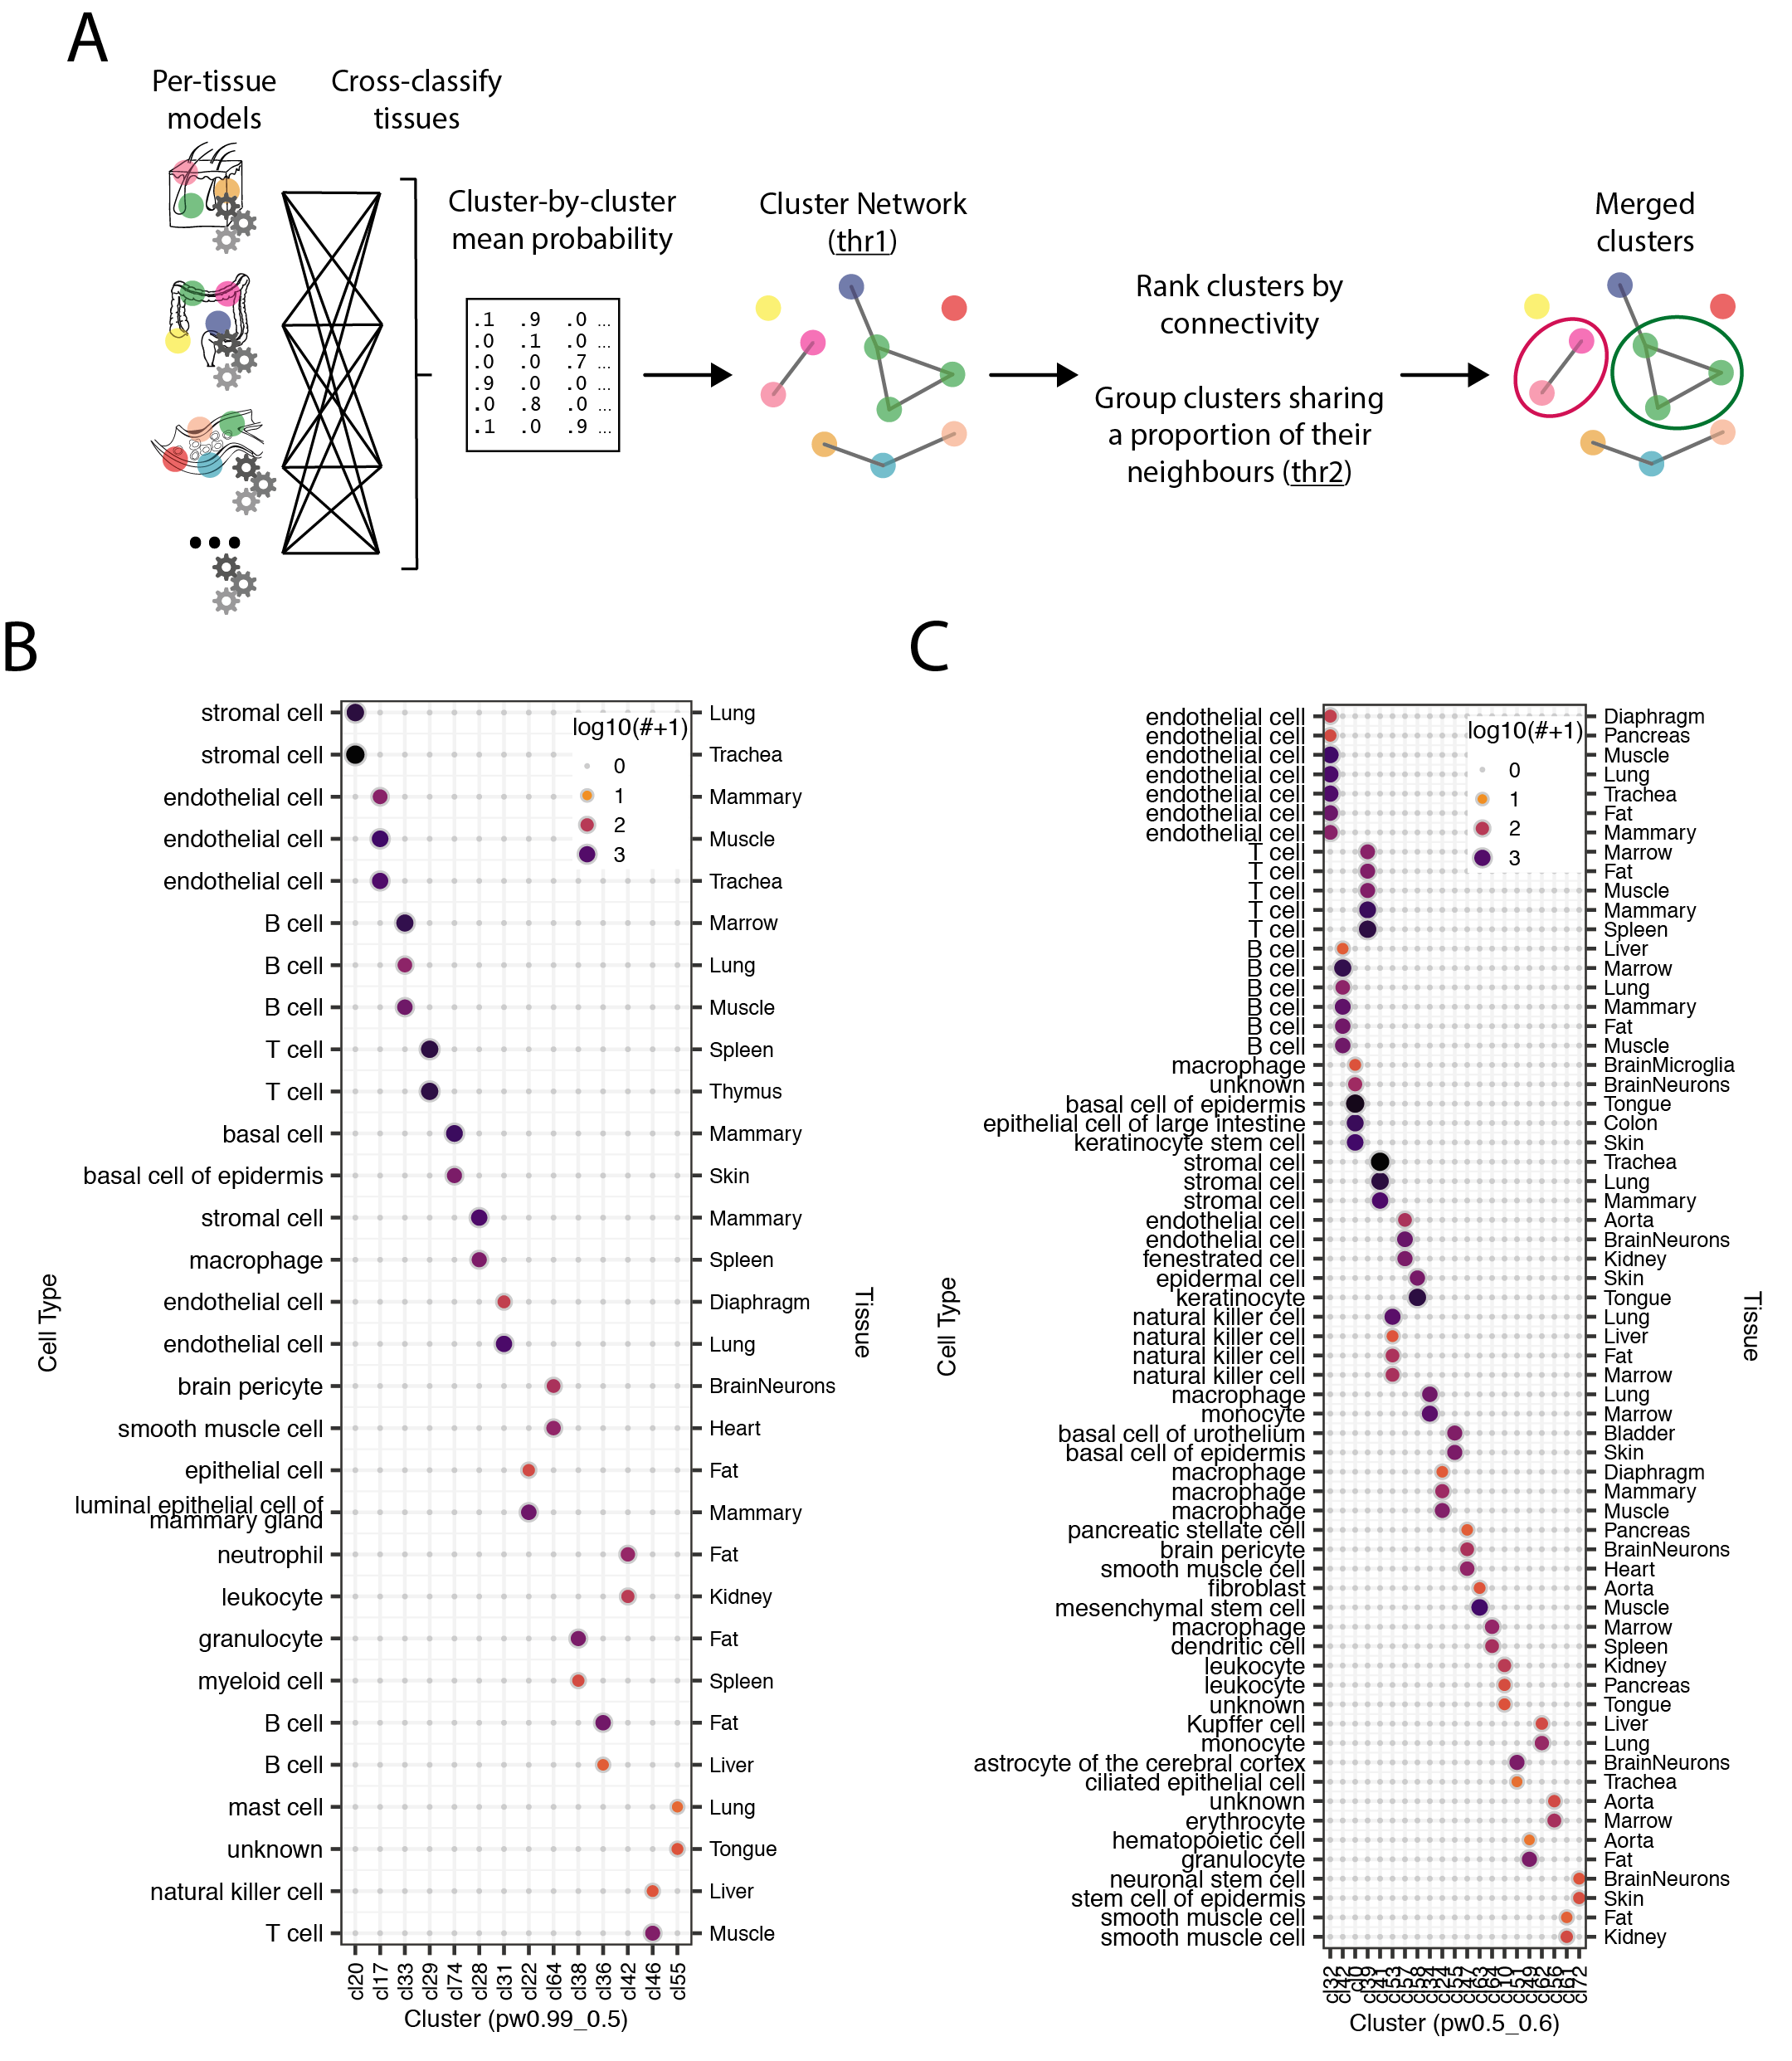
\includegraphics[width=1.0\textwidth]{Chapter3/Figs/chap3_combineClusters.png} % change word in curlies to change figure
    \caption[Cross-tissue matching of cell types]{\textbf{Cross-tissue matching of cell types}\newline\textbf{(A)} For each tissue, a logistic regression model is trained, and used obtain a classification probability of all tissues. Clusters are then linked depending on the mean probabilities of one cluster matching another (\textit{thr1}). Clusters are ranked on connectivity, and grouped with neighbouring clusters that share a proportion of its neighbours (\textit{thr2}). (Continued on the following page.)}
    \label{fig:chap3_combcl}
\end{figure}
\begin{figure}[t]
  \contcaption{(continued) \textbf{(B and C)} Merging of cell types (x-axis) using the method in (A) for models trained on known cell type labels (left y-axis). \textbf{(B)} shows the top parameter combination (thr1 = 0.99, thr2 = 0.5) based on split-join distance; \textbf{(C)} shows the combination that came in third (thr1 = 0.5, thr2 = 0.6) and which resulted in increased merging.}% Continued caption
\end{figure}

% B and C - testing using the cell types as labels - what cell types get merged?
To test how this algorithm performed in a situation with known labels, it was tested using the annotated cell types for each tissue instead of clusters. After ranking the solutions given by the different parameter combinations tested (combinations identical to Figure~\ref{fig:chap3_combdat}B), we inspected the top parameter combination (Figure~\ref{fig:chap3_combcl}B, thr1 = 0.99 and thr2 = 0.5), as well as the third, which presented the lowest combined cluster number (Figure~\ref{fig:chap3_combcl}C, thr1 = 0.5 and thr2 = 0.6). Most clusters resulting from the merging workflow, in both solutions, combined cell types annotated with the same name in different tissues. This is particularly evident for endothelial cells, B cells, and T cells. While the score for the merging  presented in panel C was not as good as that for panel B, it is immediately apparent that the more extensive merging still conserves most of the correct labeling, even grouping together identical cell types that are left separate in the first solution. This indicates that there can be a range of approximately correct parameter combinations, and hints at the tissue specificity of certain widespread cell types. Taking as an example endothelial cells, the first combination leaves lung and diaphragm separate from the remaining tissues.

% how it looks with clusters
This merging was then performed on the tissue clusters obtained in the first section of the pipeline. Both thresholds in the algorithm were tested with the values 0, 0.1, 0.2, 0.25, 0.3, 0.4, 0.5, 0.6, 0.7, 0.75, 0.8, 0.9, and 0.99. With the increase of both parameters, we observe an increase in the total number of clusters and a decrease in the fraction of merged clusters (Figure~\ref{fig:chap3_combdat}A). This trend is more evident for thr2, which is more directly involved in determining which clusters are kept together. Parameter combinations were then ranked based on their reduction of the split-join distance when comparing with known cell type labels, taking the original per-tissue clusters as a baseline. The parameter grid (Figure~\ref{fig:chap3_combdat}B) shows lower values for this ratio at higher thr2 values, with the top combination at thr1 = 0.8, thr2 = 0.99. Examining this combination for how cell type labels were grouped revealed that, similarly, to Figure~\ref{fig:chap3_combcl}B and C, many similar cell types had been grouped together (e.g. T cells; endothelial cells). Moreover, we can observe that cells with different names but similar functions are grouped together, as is the case of endothelial cells and fenestrated cells (an endothelial cell part of the renal glomerulus). In contrast, however, it could be observed that some cell types dispersed across more than one cluster. Even so, in cases where this happened (e.g. kidney tubule cell; mesenchymal stem cell of adipose), this dispersion tended to be minor, with a majority of cells from each of these annotated cell types coalescing in one cluster.

In sum, this demonstrates that this workflow is capable of merging cells with a similar transcriptome, and making cell identity across tissues uniform.


\subsection{Model training and evaluation}
\label{section3.2.3}

\begin{figure}[ht!] % LAST FIGURE FROM NEXT SECTION (PLACED HERE FOR FORMATING)
    \centering    
    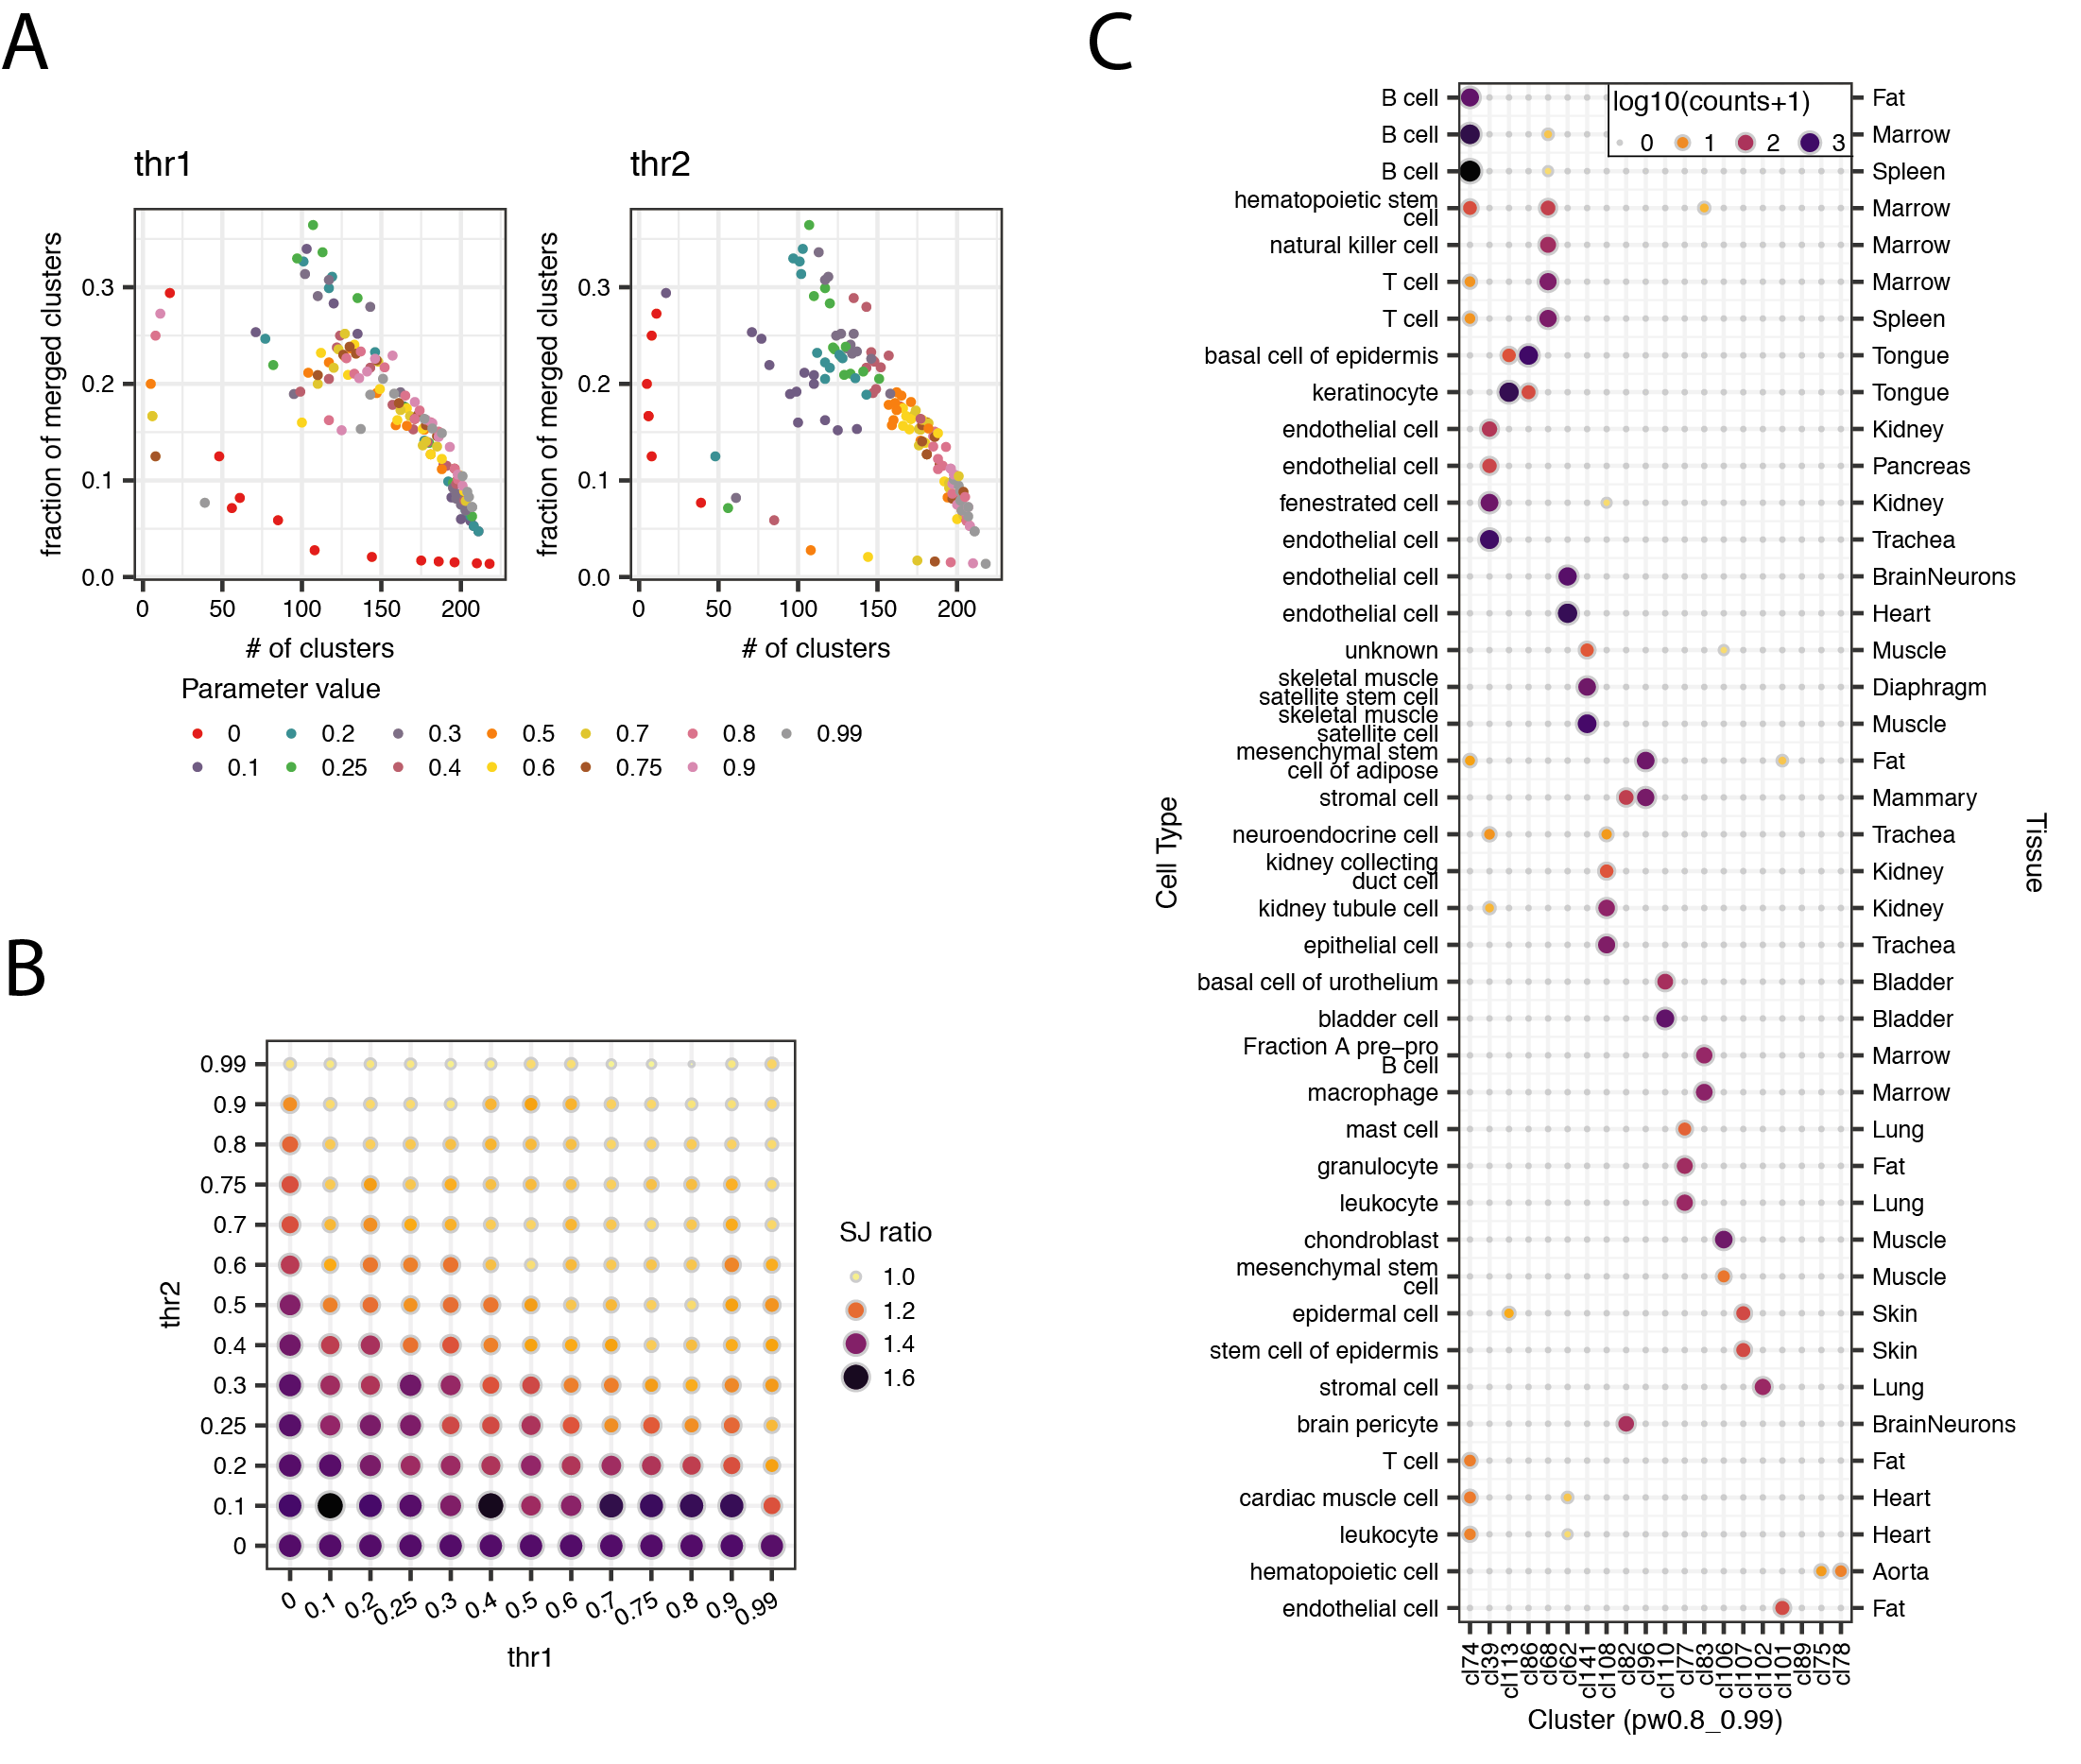
\includegraphics[width=1.0\textwidth]{Chapter3/Figs/chap3_combineData.png} % change word in curlies to change figure
    \caption[Evaluation of clusters matched across tissues]{\textbf{Evaluation of clusters matched across tissues}\newline\textbf{(A)} Change in number of total clusters and fraction of merged clusters with each threshold value (see Figure~\ref{fig:chap3_combcl}A for reference). Parameters resulting in a single cluster were not represented. \textbf{(B)} Parameter grid showing the variation of the ratio of split-join distance between merged clusters and cell type annotation, and per-tissue clusters and cell type annotation. \textbf{(C)} Grouping of cell types contained in per-tissue clusters (x-axis) using the top parameter combination (thr1 = 0.8, thr2 = 0.99) based on split-join distance.}
    \label{fig:chap3_combdat}
\end{figure}

\begin{figure}[ht!]
    \centering
    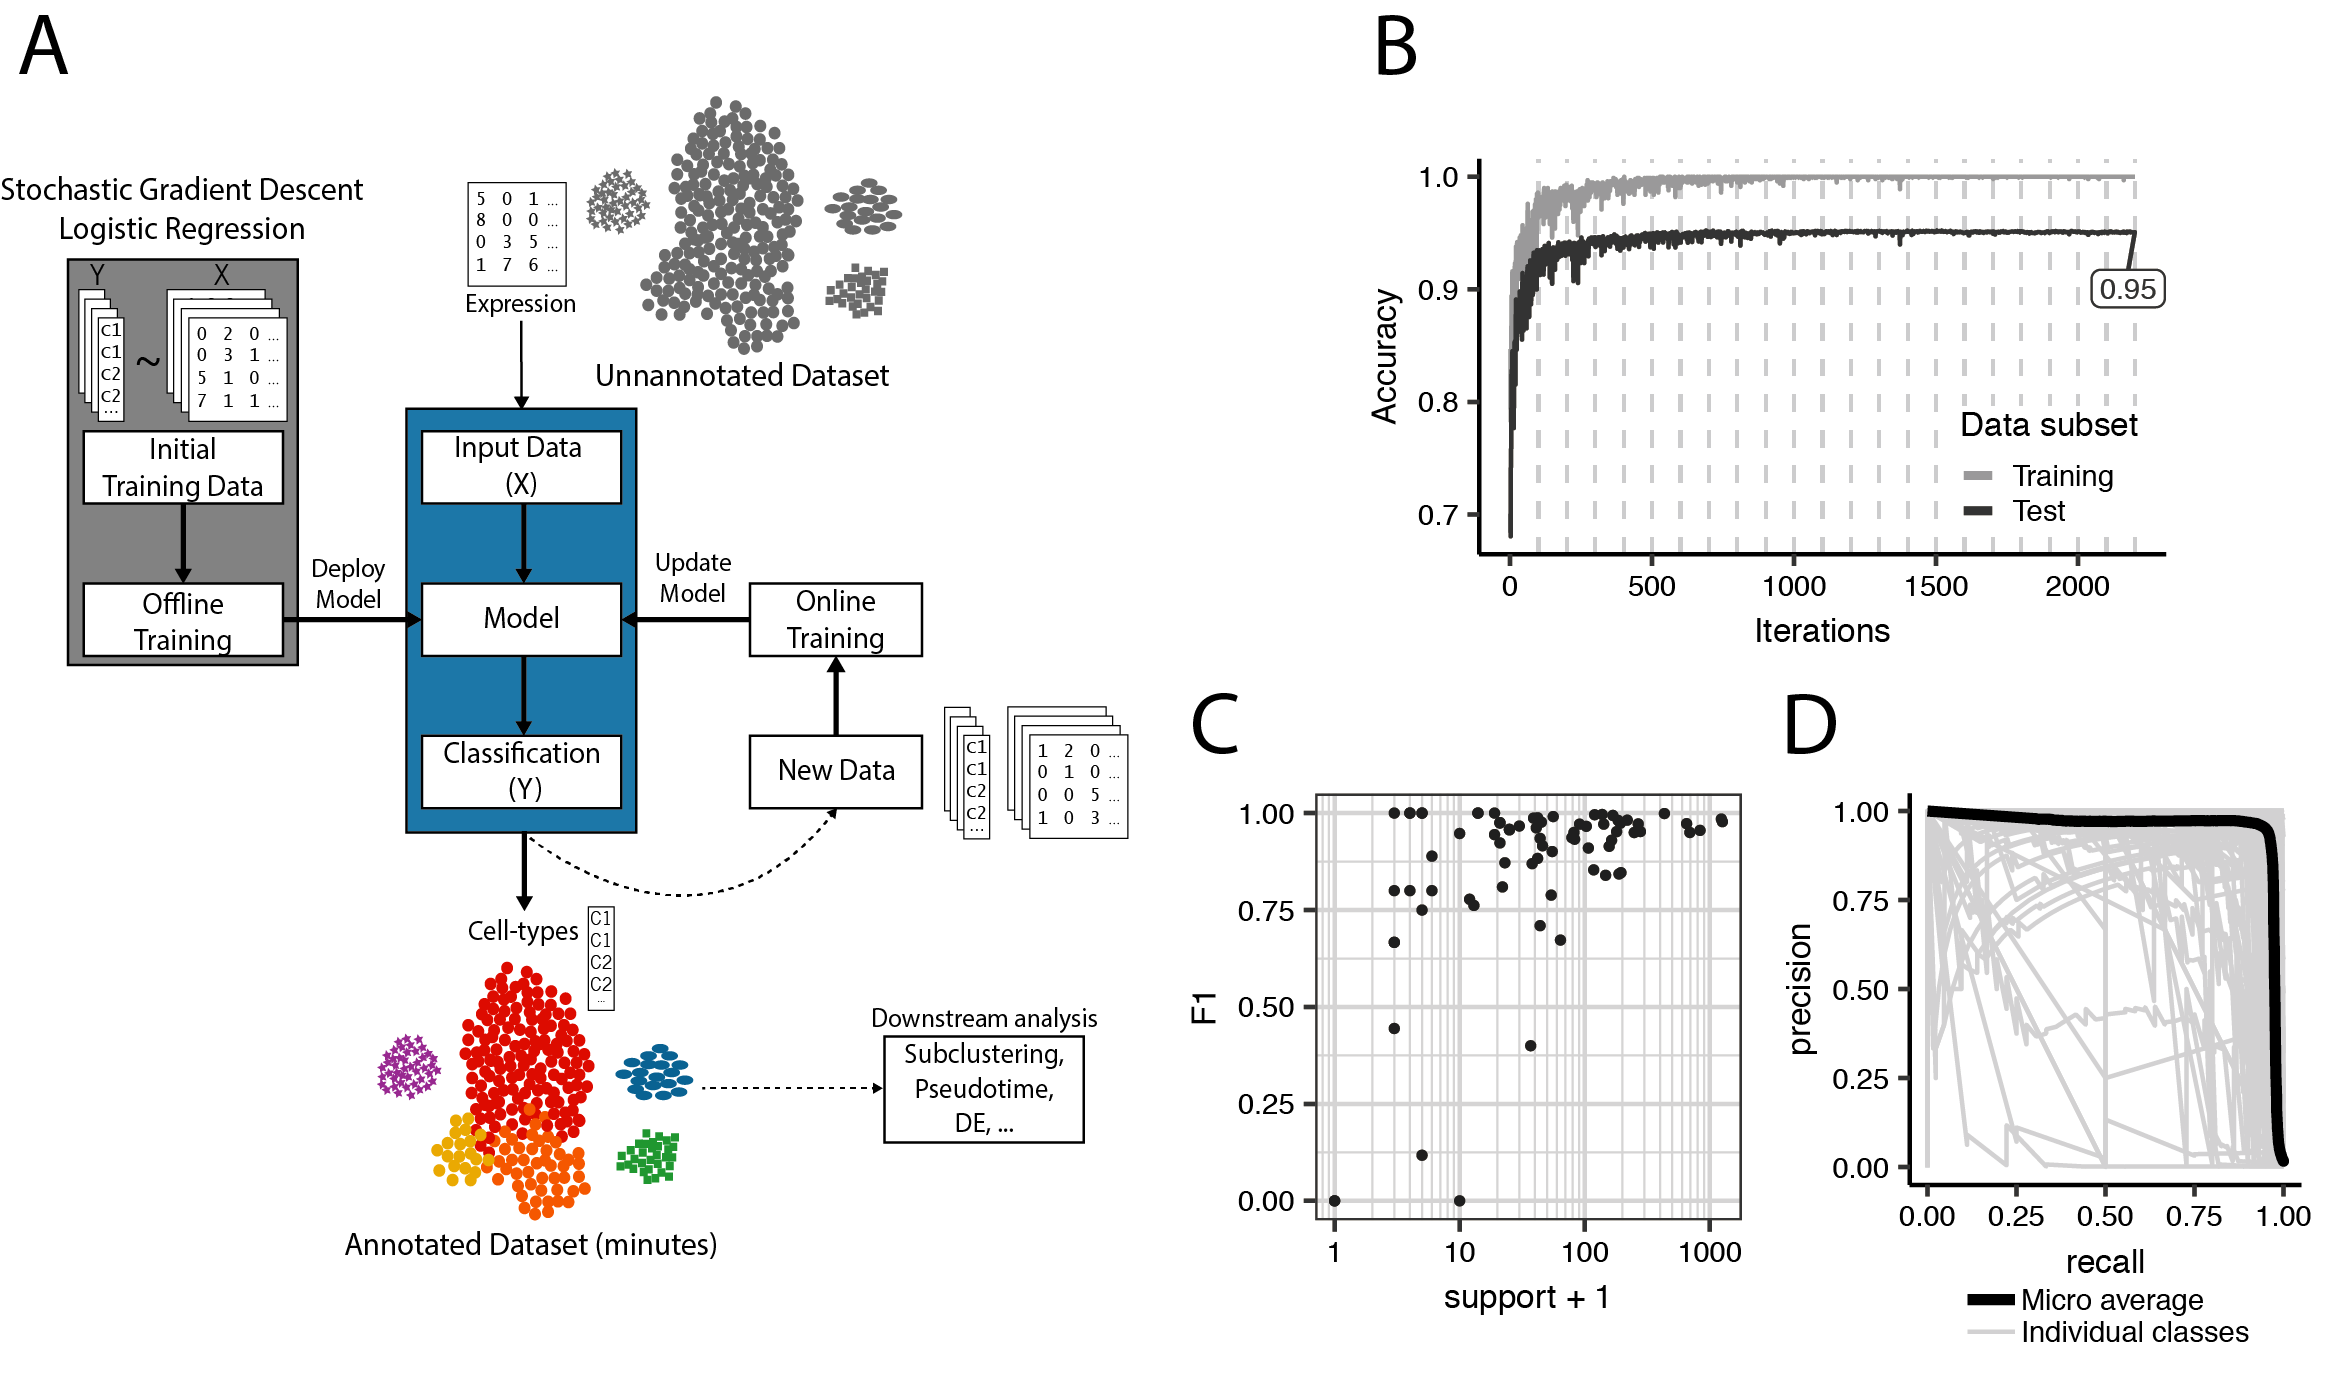
\includegraphics[width=1.0\textwidth]{Chapter3/Figs/chap3_model.png} % change word in curlies to change figure
    \caption[Model training outline and evaluation]{\textbf{Model training outline and evaluation}\newline\textbf{(A)} Model training and usage outline. A logistic regression model is trained using stochastic gradient descent. When deployed, it can provide annotations for unlabelled data, which can the be further supplied back into the model to update it. \textbf{(B)} Accuracy during model fitting for training and held-out test data, to directly predict \textit{Tabula Muris} cell type labels. Vertical dashed lines represent each training epoch. Terminal label indicated final accuracy for prediction in the test set. \textbf{(C)} F1-score for each cell type (black dots) as a function of class size (in log10 scale). \textbf{(D)} Precision-curves for each cell type (gray), and global micro average (black).}
    \label{fig:chap3_model}
\end{figure}

% explain models, mention how the per-tissue and global models were trained
The last step in \textit{CellTypist} is training the classifier. The goal of the classifier is to provide a fast and unbiased cell identity annotation of new datasets (Figure~\ref{fig:chap3_model}A). \textit{CellTypist}'s classifier is implemented in Python using scikit-learn~\citep{scikit-learn}, and uses a logistic regression model with L2 regularization. This allows the model to remain accurate, while still providing information about the contribution of all genes to determining the classification of each cell type. Training is done through mini-batch training using stochastic gradient descent (SGD). SGD is used since it makes the model more scalable, as it can converge without training over the whole dataset. It requires approximately one million data points to train, provided that all observations from all labels are passed to it. The the models here presented, will see the whole data a fixed number of times (epochs), to demonstrate their behaviour during training. The model encompassing all tissues was trained for 25 epochs, and the models trained on individual tissues (used in~\ref{section3.2.2}, Figure~\ref{fig:chap3_combcl}) were trained for 10 epochs. Additionally, SGD also allows for online training, meaning that if new data is obtained it can be easily incorporated into the model.

\begin{figure}[ht!]
    \centering    
    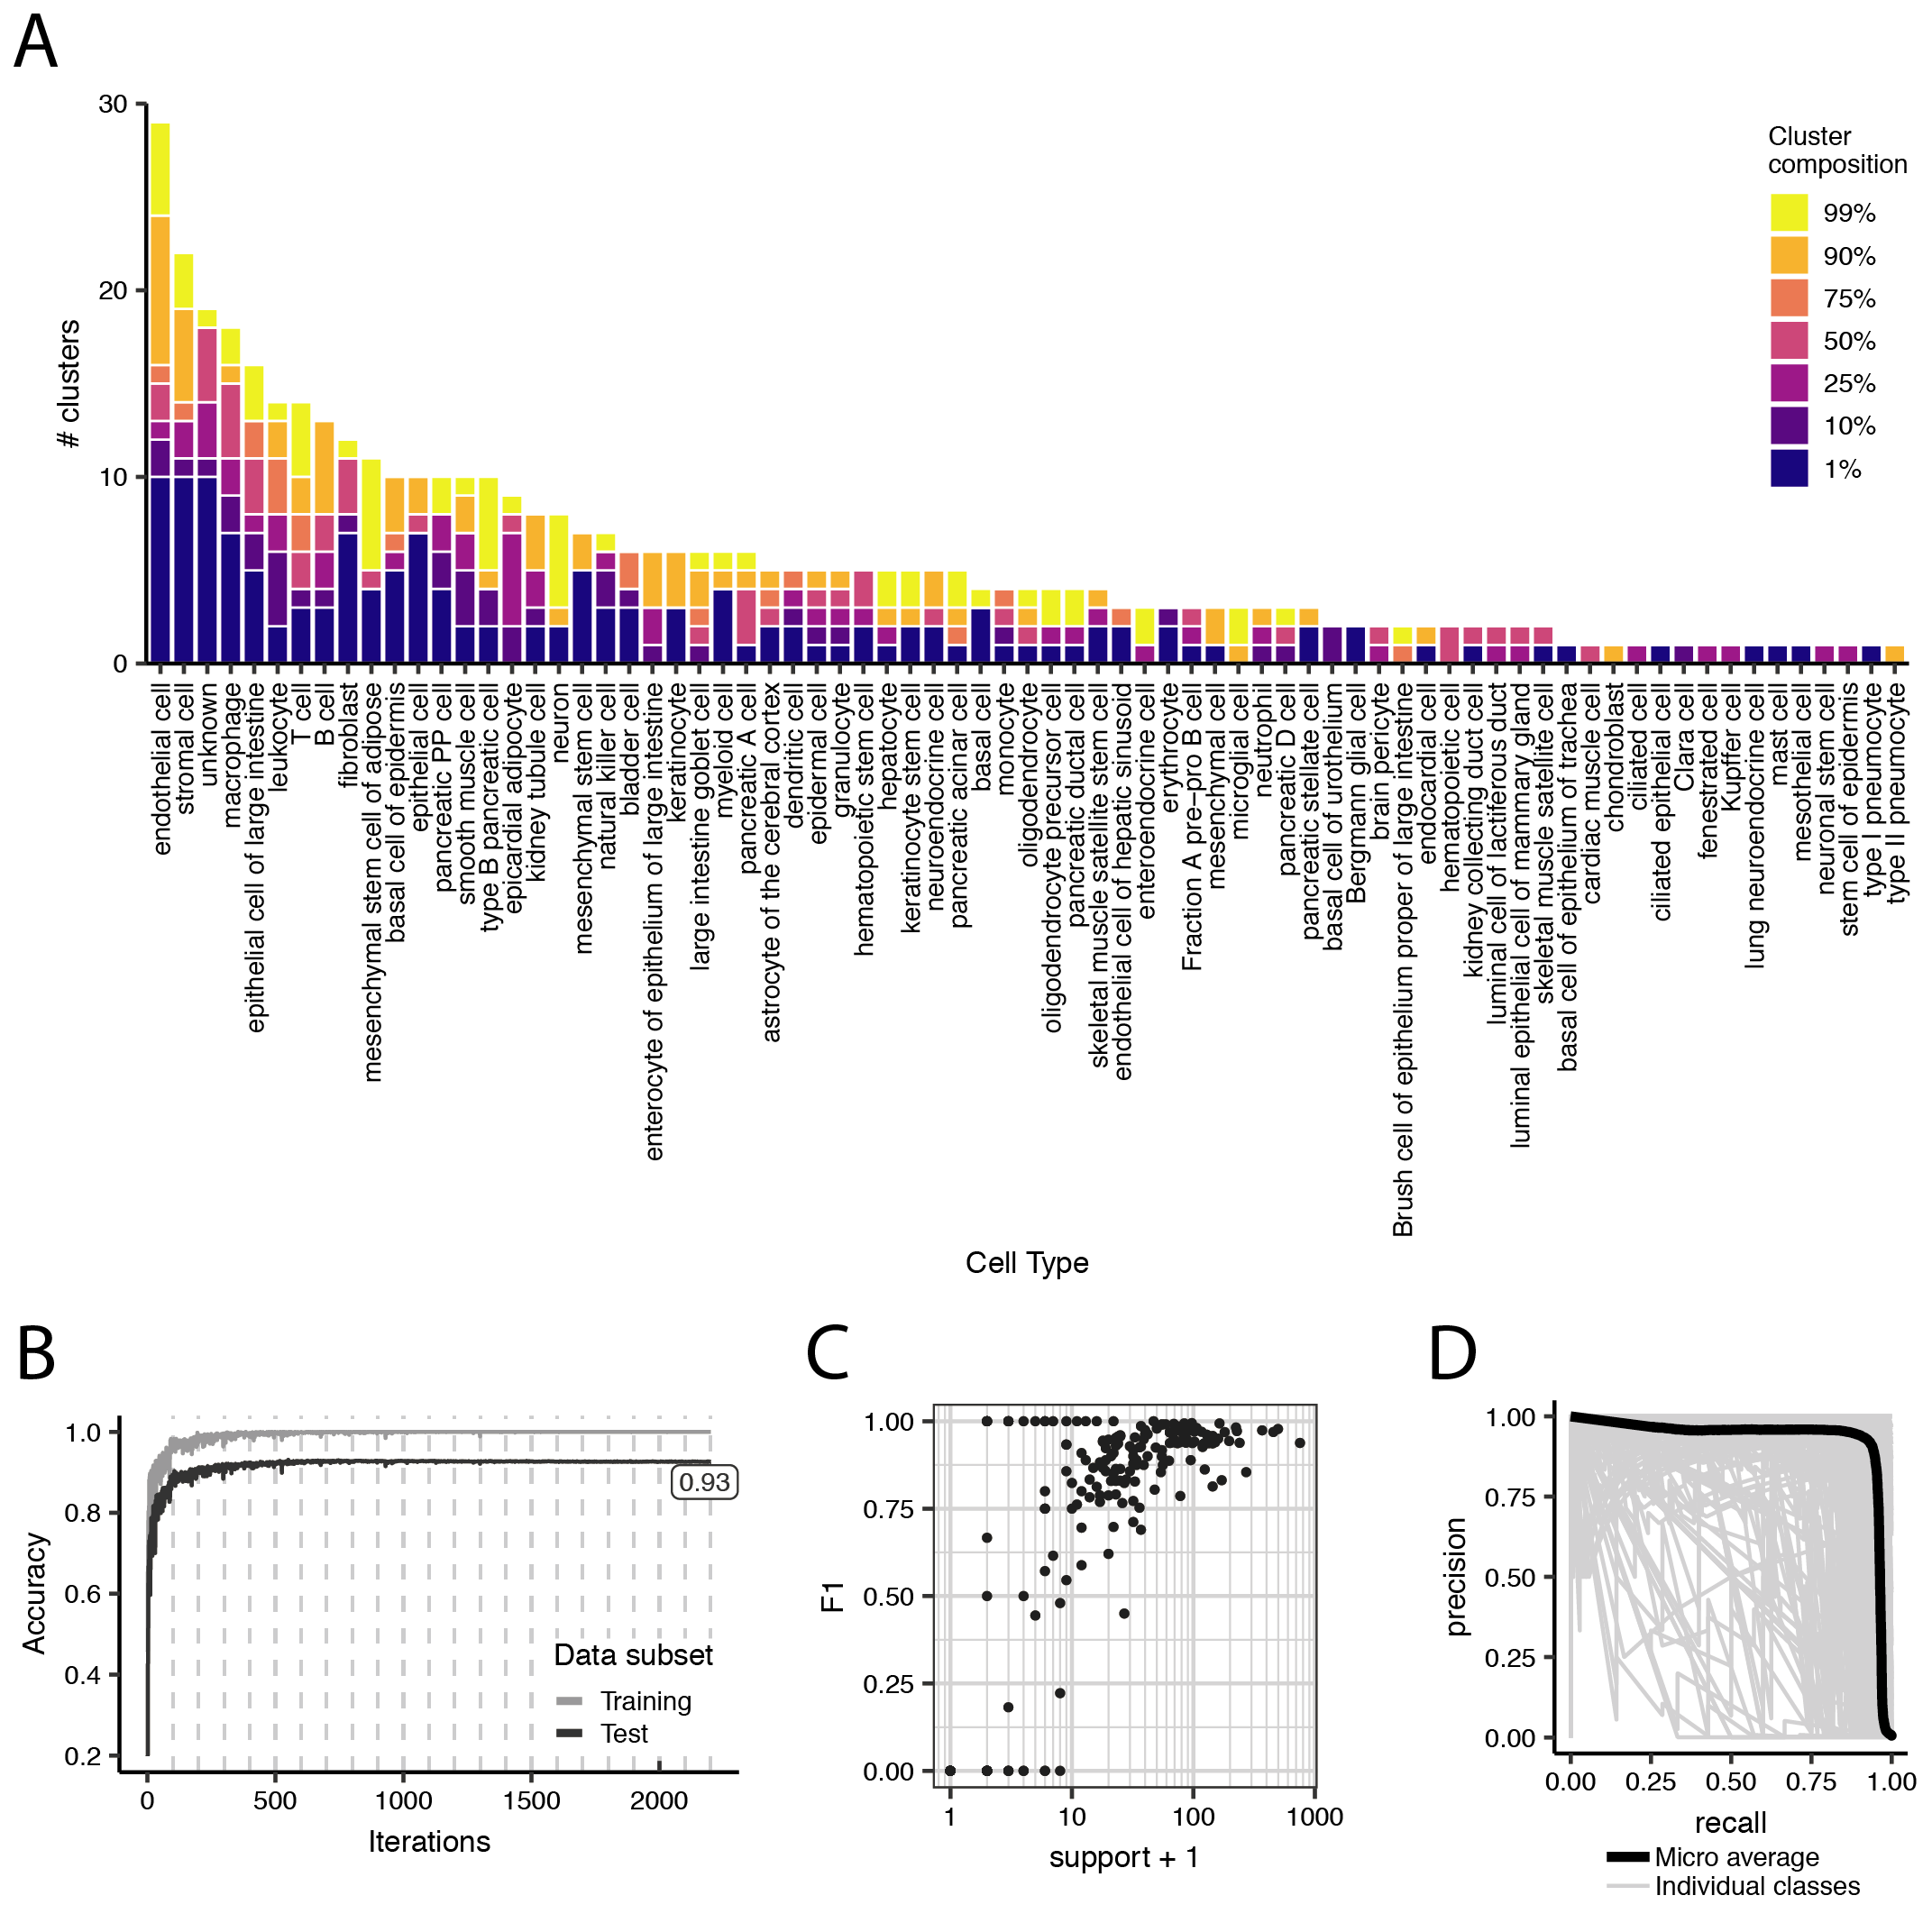
\includegraphics[width=1.0\textwidth]{Chapter3/Figs/chap3_modelcl.png} % change word in curlies to change figure
    \caption[Evaluating model trained on cross-tissue integrated clusters]{\textbf{Evaluating model trained on cross-tissue integrated clusters}\newline\textbf{(A)} Abundance of annotated cell types in cross-tissue clusters. Colours represent clusters with at least x\% of a given cell type. \textbf{(B)} Accuracy during model fitting for training and held-out test data, to predict cross-tissue integrated clusters. Vertical dashed lines represent each training epoch. Terminal label indicated final accuracy for prediction in the test set. \textbf{(C)} F1-score for each cluster label (black dots) as a function of class size (in log10 scale). \textbf{(D)} Precision-curves for each cluster (gray), and global micro average (black).}
    \label{fig:chap3_modelcl}
\end{figure}

This methodology was tested on the complete \textit{Tabula Muris} dataset, training the model to predict the existing cell type annotations. The model converged after fewer than 500 iterations (each iteration corresponding to a batch of 1000 cells), and resulted in a prediction accuracy of 95\% on the held-out test set (Figure~\ref{fig:chap3_model}B). Performance per class was assessed by calculating the F1 score, i.e. the harmonic mean between precision and recall for each class. A partial dependency between this score and the number of cells in a give class was observed for smaller groups (fewer than 100 cells, Figure~\ref{fig:chap3_model}C). The strong predictive capability of the model can be further observed by plotting the precision-recall curves for each class (Figure~\ref{fig:chap3_model}D). While we again observe some classes to have a poorer performance, a micro-averaging of precision and recall of all classes (i.e. average precision and recall by calculating true positives, false positives and false negatives for each class) shows a very strong performance.

The model training framework was further tested using the cluster labels resulting from the merging shown in Figure~\ref{fig:chap3_combdat} (thr1 = 0.8, thr2 = 0.99). Figure~\ref{fig:chap3_modelcl}A examines the representation of annotated cell types across all clusters, showing that a large majority of cell types are in one or more clusters where they represent at least 90\% of cells. Similarly to the cell type-based model, performance metrics globally show a fast convergence and high training accuracy (Figure~\ref{fig:chap3_modelcl}B), as well as a high per-label precision and recall (Figure~\ref{fig:chap3_modelcl}C, D), with most classes having an F1 score above 0.75.

These results demonstrate the high performance of simple and intuitive logistic regression to train models capable of annotating data from various sources.


\nomenclature[z-SGD]{SGD}{Stochastic Gradient Descent}

\section{Discussion}
\label{section3.5}
\textit{CellTypist} has been designed as a way of systematising cell identity from expression data, and use it directly for automatic annotation. The pipeline has been designed keeping scalability in mind, fully aware that the first model represents an initial release that will be continuously updated. It is expected that the increase in data sources and available expert annotations will greatly improve the usability of the framework going forwards.

The construction of the \textit{CellTypist} pipeline is also subject to evolution. It has been developed with the ability to include unannotated data in a cell type reference. Existing cell type annotation is highly informative when deposited together with the expression data or the accompanying publication, although this is not always the case. Even so, the vast majority of scRNA-seq analysis pipelines rely either on Leiden~\citep{traag_louvain_2019} or Louvain~\citep{blondel_fast_2008} clustering, which are used in the per-tissue processing step and thus results in a considerable approximation between known and new labels (Figure~\ref{fig:chap3_pertiss}B). Even though the final, merged labels can be manually curated and named, existing cell type annotations can also be made available to the end user, adding another layer of validation to the results.

The results here presented demonstrate that integration using the pipeline correctly merges similar cell types (Figures~\ref{fig:chap3_combcl}B,C and~\ref{fig:chap3_combdat}C). However, these results are not perfect. Figure~\ref{fig:chap3_combdat}C shows that the merged clusters are composed of more than one annotated cell type, and can at times include cells with unrelated annotations. This unexpected mixing is not a result of the cluster matching procedure, but rather a product of the initial per-tissue clustering step (Figure~\ref{fig:chap3_pertiss}C). The initial step combining datasets is thus crucial to obtain clusters representing specific cell types with high purity, while retaining as much cell type/state specificity as possible. The fact that, in some instances, T cells share clusters with natural killer cells, is an example that the method does not yet achieve perfect cell type separation. These two cell types have similar transcriptomes, which explains why in some reduced representations used for clustering they might appear very close. Nonetheless they are easily distinguishable by the expression of a small set of markers, and can thus be efficiently distinguished by a logistic regression model (Figure~\ref{fig:chap3_model}C and D). 

The resolution bottleneck introduced by the first, per-tissue integration step can be potentially improved in a few ways. One possibility is to adopt a more curated approach after clustering every tissue, although this would require significantly more human input. Another option would be to rely more on data with existing annotations. One way to achieve this is by using a label propagation method that, within each integrated tissue, passes existing labels to unannotated data~\citep{barkas_joint_2019}. Alternatively, the method can instead iteratively apply the algorithm used to integrate the clusters between tissues (Figure~\ref{fig:chap3_combcl}A). In the first step this would be applied for each dataset collected to merge all existing data for each tissue, and relying on existing annotations. A second step would then be applied between tissues as shown (Figure~\ref{fig:chap3_combcl}). This guarantees that any known heterogeneity in the collected data is preserved and propagated into the final annotation, but has the disadvantage that any novel populations that would be detected by data integration can be lost.

This Chapter also demonstrated the viability of logistic regression as a methodology for cell type classification using a broad atlas as a reference (Figures~\ref{fig:chap3_model}B-D and~\ref{fig:chap3_modelcl}B-D). This is in line with previous reports~\citep{kohler_deep_2019,abdelaal_comparison_2019}, showing that cell identity classification is not improved by the use of deep learning methods, and can be accurately performed using simpler machine learning frameworks. The results here also demonstrate that this method is robust enough to accommodate clusters with some mixture of cell types (which results in lower phenotypic resolution) (Figure~\ref{fig:chap3_modelcl}C).

The implementation of \textit{CellTypist} is also explicitly constructed such that the resulting model can be easily updated. This is due to the implementation using stochastic gradient descent, which allows for easy and direct updates to the model by running more learning iterations on novel data. This is important to maintain the reference up to date. However, it can only be done by classifying new data according to the existing labels. If the new datasets collected include cell types that are not represented in \textit{CellTypist}, then the full pipeline needs to be ran anew. Nonetheless, this allows for the database to have fast minor releases to maintain it up to date with the latest dataset publications, as well as less frequent major releases that more thoroughly integrate these datasets and revise the annotation database. \textit{CellTypist} will be available with a web interface, allowing for classifications to be ran via a web server, or, alternatively, download the models to test locally. It will include a database characterising the cell type labels present in the model. While different organisms will have different models, many of the cell types described are predicted to be present in multiple species, and can in future updates have their cross-species similarities defined and reflected in \textit{CellTypist}'s accompanying cell type compendium.

% usefulness (will be demonstrated in the next chapter)
Overall, this chapter has demonstrated that \textit{CellTypist} can organise a valuable resource for cell type annotation. Furthermore, this resource can be readily interpreted from inspection of gene coefficients for each label. In the next chapter, a practical application and interpretation of \textit{CellTypist} using human data will be presented.